\documentclass[a4paper,11pt]{article}
\usepackage{filecontents}

\usepackage[utf8]{inputenc}
\usepackage[english]{babel}
\usepackage{graphicx, array, blindtext}
\usepackage[colorinlistoftodos]{todonotes}
\DeclareUnicodeCharacter{2212}{-}
\usepackage [a4 paper , hmargin = 1.2 in , bottom = 1.5 in] {geometry}
\usepackage [parfill] {parskip}

\usepackage{enumitem}
\usepackage{amsmath}
\usepackage{amsthm}

\usepackage{nameref}
\usepackage{amssymb}
\usepackage [linesnumbered, ruled, vlined] {algorithm2e}
\usepackage{listings}
\usepackage{xcolor}
\usepackage{floatrow}
\usepackage{siunitx}


\usepackage{cancel}
\usepackage{fancyhdr}
\usepackage{graphicx}
\usepackage{verbatim}
\usepackage[document]{ragged2e}

\renewcommand{\footrulewidth}{0.4pt}
\newtheorem{definition}{Definition}
\numberwithin{definition}{section}
\newtheorem{mytheorem}{Theorem}
\numberwithin{mytheorem}{subsection}
\newcommand{\notimplies}{\;\not\!\!\!\longrightarrow}  
\newcommand\norm[1]{\left\lVert#1\right\rVert}
\pagestyle{fancy}
\fancyhf{}
\rhead{CS754 Assignment 1}
\lhead{200050013-200050130}
\fancyfoot[C]{Page \thepage}
\usepackage{subcaption}
\usepackage{listings}


\usepackage{hyperref}
\urlstyle{same}
\hypersetup{pdftitle={main.pdf},
    colorlinks=false,
    linkbordercolor=red
}
\usepackage{array}
\usepackage{listings,chngcntr}

\begin{document}
\centering{

\title{\fontsize{150}{60}{CS754 Assignment 1 Report}}

\author{
Arpon Basu \\ Shashwat Garg }
}

\date{Spring 2022}
\maketitle

\justifying
\tableofcontents

\newpage
\justifying
\section*{Introduction}

Welcome  to our report on CS754 Assignment 1. We have tried to make this report comprehensive and self-contained. We hope reading this would give you a proper flowing description of our work, methods used and the results obtained. Feel free to keep our code scripts alongside to know the exact implementation of our tasks. 

We have referred to some sites on the web for finding the MATLAB implementations (generic documentation pages) and the same has been added in the references section. 

In many places, to better give context to the place from which the questions could have arisen, some theoretical discussions have been engaged in.

Hope you enjoy reading the report. Here we go!




\newpage
\section{Problem 1}
We have been given the following problem-

Let $\boldsymbol{\theta^{\star}}$ : $\textrm{min} \|\boldsymbol{\theta}\|_1$ such that $\|\boldsymbol{y}-\boldsymbol{\Phi \Psi \theta}\|_2 \leq \varepsilon$, where $\boldsymbol{x} = \boldsymbol{\Psi \theta}$ and $\boldsymbol{y} = \boldsymbol{\Phi x} + \boldsymbol{\eta}$. $\varepsilon$ is an upper bound on the magnitude of the noise vector $\boldsymbol{\eta}$.

Also, Theorem 3 states-\\If $\boldsymbol{\Phi}$ obeys the restricted isometry property with isometry constant $\delta_{2s} < \sqrt{2}-1$, then we have $\|\boldsymbol{\theta} - \boldsymbol{\theta^{\star}}\|_2 \leq C_1 s^{-1/2}\|\boldsymbol{\theta}-\boldsymbol{\theta_s}\|_1 + C_2 \varepsilon$ where $C_1$ and $C_2$ are functions of only $\delta_{2s}$ and where $\forall i \in \mathcal{S}, \boldsymbol{\theta_s}_i = \theta_i; \forall i \notin \mathcal{S}, \boldsymbol{\theta_s}_i = 0$.

\subsection{Trend of Error Bound with $s$}
This is not a discrepancy. In reality, we are ignoring the change in $C_1$ and $C_2$. The point is, we are only focusing on the effect of $s^{-1/2}$ and $||\boldsymbol{\theta}-\boldsymbol{\theta_s}||_1$. We must also see the changes in $C_1$ and $C_2$, which increase as the value of $\delta_{2s}$ changes.

As the value of $s$ increases, due to reducing sparsity, we observe that (the bound on) $\delta_{2s}$ also increases. Intuitively, this is because an increase in $s$ implies an increase in the required number of linearly independent columns required in the $\boldsymbol{\Phi \Psi}$ matrix. This is unlikely as s increases. An increase in $\delta_{2s}$ leads to an increase in the value of $C_1$ and $C_2$.

Thus we have two opposing behaviors and we cannot claim that the error bound improves as the sparsity measure, $s$ increases in value.

\subsection{Dependence of error bound on $m$}

$m$ does not directly affect the error bound but it has several other indirect implications. 

First of all, we require our matrix $\boldsymbol{A}=\boldsymbol{\Phi \Psi}$ to obey the RIP, for which we usually construct our sensing matrix $\boldsymbol{\Phi}$ using Gaussian or Bernoulli entries randomly. The probablility that this happens is very high in case $m \geq CS \log(n/S)$.

Apart from this, $m$ also affects the value of $\epsilon$ which we can take in case of uniform Gaussian noise in the measurements. In such cases, a good approximation of $\epsilon$ is given by 3 standard deviations around the mean, which effectively translates into $\epsilon \geq 9m\sigma^2$.

Finally, when $m$ increases, we observe that the rank of the matrix $\boldsymbol{A}$ increases, which would make it satisfy the RIP with a higher probability. This would indicate a drop in the value of $\delta_{2s}$, indicating a drop in the constants $C_1$ and $C_2$ and thus improving the error bound.

Thus, m has a lot of indirect implications in the error bound.

\subsection{Change in requirement of $\delta_{2s}$}

Theorem 3 is better than Theorem 3A. Theorem 3 provides the same guarantees for more relaxed values of $\delta_{2s}$.

For large $\delta_{2s}$ we can work with comparatively less sparse signals. For values of $\delta_{2s} \geq 0.1$, Theorem 3A doesn't guarantee anything while the Theorem 3 works well for all values till 0.4142.

Also, for values of $\delta_{2s} \leq 0.1$, both the theorems give the exact same reconstructions.

Thus, Theorem 3 is much more useful.


\subsection{Setting $\epsilon = 0$}

This is not the correct way to solve the problem in presence of noise.

By setting the $\epsilon$ to 0, we have ignored the noise and thus our $\theta$ obtained from such a method will be incorrect. We might encounter several problems. We might not be able to converge on a value, because a solution does not even exist in this case of constraints. We might overfit our measurements to include noise which would result in the $\theta$ not being the sparsest and correct measurement.

Instead, we should choose an $\epsilon$ greater than the noise magnitude, for good results.



\newpage


\section{Problem 2}
We note that this problem has two parts: One for demonstrating that the upper bound of $\mu(\boldsymbol{\Phi, \Psi})$ is $\sqrt{n}$, and one for demonstrating that the lower bound of $\mu(\boldsymbol{\Phi, \Psi})$ is 1. We shall deal with both parts separately.\\
\subsection{Lower Bound}
\begin{proof}
Since $\boldsymbol{\Psi}$ is an orthonormal matrix, it's column vectors $\boldsymbol{\Psi_1}$, $\boldsymbol{\Psi_2}$, ..., $\boldsymbol{\Psi_n}$ form a orthonormal basis for $\mathbb{K}^n$, and consequently we can express $\boldsymbol{g}$ as $\sum_{k=1}^{n} \alpha_k\boldsymbol{\Psi_k}$. Also, $\lVert \boldsymbol{g}\rVert_2 = \sqrt{\sum_{j=1}^{n} \alpha^2_j}$, following which we get $\boldsymbol{g}_{\mathrm{normalized}} = \sum_{k=1}^{n} \frac{\alpha_k}{\sqrt{\sum_{j=1}^{n} \alpha^2_j}}\boldsymbol{\Psi_k}$. Thus $\mu(\boldsymbol{g, \Psi)} = \sqrt{n}\cdot\mathrm{max}_{i\in[n]}\;|\boldsymbol{g}_{\mathrm{normalized}}^T\boldsymbol{\Psi_i}| = \sqrt{n}\cdot\mathrm{max}_{i\in[n]}\;\frac{|\alpha_i|}{\sqrt{\sum_{j=1}^{n} \alpha^2_j}}$. WLOG assuming that $|\alpha_1| = \mathrm{max}_{i\in[n]}\;|\alpha_i|$, we get that
$$\mu(\boldsymbol{g, \Psi}) \geq \sqrt{n}\cdot\mathrm{max}_{i\in[n]}\;\frac{|\alpha_i|}{\sqrt{\sum_{j=1}^{n} |\alpha_1|^2}} = \sqrt{n}\frac{|\alpha_1|}{\sqrt{n\alpha^2_1}} = 1$$
as desired. Note that equality is achieved iff $\alpha_1 = \alpha_2 = ... = \alpha_n$.
\end{proof}
\subsection{Upper Bound}
\begin{proof}
Directly borrowing from the previous proof, $\mu(\boldsymbol{g, \Psi)} = \sqrt{n}\cdot\mathrm{max}_{i\in[n]}\;|\boldsymbol{g}_{\mathrm{normalized}}^T\boldsymbol{\Psi_i}|$. Now, by the Cauchy Schwartz inequality, for any two vectors $\boldsymbol{u}$, $\boldsymbol{v}$, we have $|\langle \boldsymbol{u}, \boldsymbol{v}\rangle|\leq \lVert \boldsymbol{u}\rVert_2\lVert \boldsymbol{v}\rVert_2$, where $|\langle \cdot, \cdot\rangle|$ is the usual Euclidean inner product. Applying it to the coherence relation yields $|\boldsymbol{g}_{\mathrm{normalized}}^T\boldsymbol{\Psi_i}| \leq \lVert \boldsymbol{g}_{\mathrm{normalized}}\rVert_2\lVert \boldsymbol{\Psi_i}\rVert_2 = 1$, and consequently we obtain that $\mu(\boldsymbol{g, \Psi)} \leq \sqrt{n}$, as desired. Note that equality is achieved iff $\boldsymbol{g}$ is parallel to some column vector $\boldsymbol{\Psi_i}$ of $\boldsymbol{\Psi}$.
\end{proof}

\newpage
\section{Problem 3}

This is a problem based on the basic concepts of linear algebra and the concepts of basis vectors, null-space property and independent vectors.

We have a compressed measurement $y$, of the form $\boldsymbol{y} = \boldsymbol{\Phi x}$ where $\boldsymbol{\Phi} \in \mathbb{R}^{m \times n}$ is the measurement matrix and $\boldsymbol{x} \in \mathbb{R}^n, ~n \gg 2$. Consequently, $\boldsymbol{y} \in \mathbb{R}^m ~(m \ll n$). Our aim is to figure out $\boldsymbol{x}$.

\subsection{$m$ = 1}
Now observe that $\boldsymbol{\Phi}$ is essentially a row vector and $\boldsymbol{x}$ is a column vector, thus, even if only a element of x was non-zero, we still do not know which index of $\boldsymbol{\Phi}$ and $\boldsymbol{x}$ combine to give the value of $\boldsymbol{y}$, which is effectively a scalar in this case.

On the other hand, if we know the value of index, then the vector $\boldsymbol{x}$ is deducible. If the index is $i$, then the elements of $\boldsymbol{x}$ are zero for all indices $j\neq i$ and equal to $\boldsymbol{y/\Phi_i}$ for the $i^{th}$ index.

Thus, answer of the first part is NO, and the second part is YES.

\subsection{$m$ = 2}

Yes! It is possible in this case, if $\boldsymbol{x}$ has only one non-zero element.

Since $\boldsymbol{x}$ has only one non-zero entry, say index $i$, only a single column of $\boldsymbol{\Phi}$ plays a role in getting the value of $\boldsymbol{y}$.

Thus, effectively,
$$\boldsymbol{y^1} = \boldsymbol{\Phi_i^1.x^i}$$
$$\boldsymbol{y^2} = \boldsymbol{\Phi_i^2.x^i}$$

This implies that the ratio of the values in the $\boldsymbol{y}$ vector, matches the ratio of the values in some column of the $\boldsymbol{\Phi}$ matrix.

If our $\boldsymbol{\Phi}$ matrix is sufficiently randomly generated, we can always uniquely find such an index.

After that, it is just like the previous question. If the index found is $i$, then the elements of $\boldsymbol{x}$ are zero for all indices $j\neq i$ and equal to $\boldsymbol{y^1/\Phi_i^1}$ or $\boldsymbol{y^2/\Phi_i^2}$ for the $i^{th}$ index.

Again, please note that the success of this method depends on the fact that all columns of $\boldsymbol{\Phi}$ are linearly independent, which is a valid assumption given the nature of $\boldsymbol{\Phi}$.

\subsection{$m$ = 3}

Here, we have a 2-sparse $\boldsymbol{x}$ vector and 3 measurements.
Effectively, we need to solve the following linear system-

$$\boldsymbol{y^1} = \boldsymbol{\Phi_i^1.x^i + \Phi_j^1.x^j}$$
$$\boldsymbol{y^2} = \boldsymbol{\Phi_i^2.x^i + \Phi_j^1.x^j}$$
$$\boldsymbol{y^3} = \boldsymbol{\Phi_i^3.x^i + \Phi_j^1.x^j}$$

Note that we do not have any idea about which indices the $i$ and $j$ might be.\\
Just as we looked at the ratio in the previous part, here we need to look at the span of the two column vectors $\boldsymbol{\Phi_i}$ and $\boldsymbol{\Phi_j}$. If the vector $\boldsymbol{y}$ lies in the span of the two vectors, then we can find an appropriate solution to the values of vector $\boldsymbol{x}$.

But there is a problem. Note that the choice of $i$ and $j$ is not unique. We know that the $m \ll n$. Thus, given that $\boldsymbol{\Phi_i}$ is a random matrix, there is a high chance that we can choose another set of 2 vectors with indices $k$ and $l$ such that $\boldsymbol{y}$ lies in the span of $\boldsymbol{\Phi_k}$ and $\boldsymbol{\Phi_l}$.

In fact, given a large enough $n$, it is certain that there will exist 4 vectors (of dimension 3) which are linearly dependent and none of the coefficients
($\alpha_i,~\alpha_j,~\alpha_k,~\alpha_l$) is zero. This means that we will always have 2 ways of representing our $\boldsymbol{y}$ vector. This implies that, we cannot always get the $\boldsymbol{x}$ vector in this case.

Surprisingly, without knowing the indices at which x is non-zero, we cannot even generate a specific $\boldsymbol{\Phi}$ such that we would have the vector $\boldsymbol{x}$. This is because such a $\boldsymbol{\Phi}$ would require most of the columns to be zero in atleast 2 places out of 3, such that we cannot get 4 linearly dependent columns with all $\alpha_i,~\alpha_j,~\alpha_k,~\alpha_l$ as non-zero. This would ensure that there is always a unique pair of indices that calculate $\boldsymbol{y}$, but again, it is not possible in the current scenario.


\subsection{$m$ = 4}

This problem very closely resembles the null-space theorem covered in the lectures. We have a 2-sparse vector and a matrix with $m = 4$. If we can ensure that any 4 columns are linearly independent then we have a solution. 

If you are wondering about whether we might fail due to 5 such columns being linearly dependent, note that in that case, we would have a 2 column representation equal to a 3 column representation. But a 3 column representation is useless in this case. Thus, we can avoid it.\footnote{The previous case, for $m$ = 3 fails because in that case, any 4 columns are linearly dependent. Thus, we can get a 2 column representation equal to another 2 column representation, which leads to multiple solutions.}

The solution is as follows-

We assume that the matrix is of rank = 4. This implies that a unique solution exists. We follow the following algorithm.

\begin{itemize}
    \item Iterate over all pairs of columns in the matrix $\boldsymbol{\Phi}$.
    \item Check if the vector $\boldsymbol{y}$ lies in the span of the two column vectors in focus.
\end{itemize}

As long as the rank $= 4$, there exists only a single solution for the algorithm.
Otherwise, we have two 2-sparse vectors as solution. This implies that their difference ie. a 4-sparse vector lies in the null-space of $\boldsymbol{\Phi}$. This is a contradiction to our assumption. Hence proved.

Thus, the answer to this part is YES (mostly, since there is a certain randomness involved in creation of these matrices).


\newpage


\section{Problem 4}

We provide a proof for this problem below.
\begin{proof}
We set up some notation first: Let 
\begin{gather*}
    \boldsymbol{x^*} :=  \mathrm{arg\;min}\boldsymbol{_{\lVert y - Ax\rVert_2 \leq e}\;\lVert x\rVert_1} \\
    \boldsymbol{l_1 := } \mathrm{min}\boldsymbol{_{\lVert y - Ax\rVert_2 \leq e}\;\lVert x\rVert_1} \\
    \boldsymbol{f(t) := } \mathrm{arg\;min}\boldsymbol{_{\lVert x\rVert_1 \leq t}\; \lVert y - Ax\rVert_2} 
\end{gather*}
Now, we prove 3 lemmas, which when joined together will help us prove the above result.
\subsection{Claim 1: $\boldsymbol{f(t) > e}\;\forall\;\boldsymbol{t < l_1}$}
Assume for the sake of contradiction that $\boldsymbol{f(t) \leq e}$ for some $\boldsymbol{t < l_1}$. That means there exists a \textbf{minimizer} $\boldsymbol{x^{\prime}}$ such that $\boldsymbol{\lVert x^{\prime}\rVert_1\leq t < l_1}$ $\Rightarrow$ $\boldsymbol{\lVert x^{\prime}\rVert_1 < l_1}$ such that $\boldsymbol{f(t) = \lVert y - Ax^{\prime}\rVert_2 \leq e}$ by the premise of our assumption. But note that when we said $\boldsymbol{l_1 = } \mathrm{min}\boldsymbol{_{\lVert y - Ax\rVert_2 \leq e}\;\lVert x\rVert_1}$, it meant that \textbf{for all vectors} that kept the L2-norm of $\boldsymbol{y-Ax}$ below $\boldsymbol{e}$, their L1-norms were greater than $\boldsymbol{l_1}$, and for exactly one unique vector $\boldsymbol{x^*}$, was the minimum possible L1-norm $\boldsymbol{l_1}$ achieved. But note that we have now synthesized a vector $\boldsymbol{x^{\prime}}$ which manages to bound the L2-norm of $\boldsymbol{y-Ax}$ while also maintaining a L1-norm lesser than $\boldsymbol{l_1}$.\\
Thus, our premise that ``$\boldsymbol{f(t) \leq e}$ for some $\boldsymbol{t < l_1}$" is false, and consequently $\boldsymbol{f(t) > e}\;\forall\;\boldsymbol{t < l_1}$.
\subsection{Claim 2: $\boldsymbol{f(l_1) \leq e}$}
What does $\boldsymbol{f(l_1)}$ exactly signify? It denotes some minimizer $\boldsymbol{x_0}$ for which $\boldsymbol{\lVert y - Ax_0\rVert_2}$ is minimized, provided that $\boldsymbol{x_0}$ belongs to our constraint set $\{\boldsymbol{x}: \lVert\boldsymbol{x}\rVert_1 \leq \boldsymbol{l_1}\}$. Now, note that $\boldsymbol{x^*}$ is a member of our constraint set since $\boldsymbol{\lVert x^\rVert_1 = l_1 \leq l_1}$, because $\boldsymbol{x^*}$ was the argument for which the L1-norm $\boldsymbol{l_1}$ was achieved. We also know that $\boldsymbol{\lVert y - Ax^\rVert_2 \leq e}$ by the very definition of $\boldsymbol{x^*}$. Thus, since one member of our constraint set assigns to $\boldsymbol{y-Ax}$ a L2-norm $\leq$ $\boldsymbol{e}$, $\boldsymbol{f(l_1)}$, which is basically the minimum of $\boldsymbol{\lVert y - Ax\rVert_2}$ over our constraint set, the minimum will obviously be $\leq$ the value for any witness, in this case $\boldsymbol{x^*}$.
\subsection{All minimizers of $\boldsymbol{\lVert y - Ax\rVert_2}$ over $\{\boldsymbol{x}: \lVert\boldsymbol{x}\rVert_1 \leq \boldsymbol{l_1}\}$ have L1-norm $\boldsymbol{l_1}$}
This claim follows naturally, since $\{\boldsymbol{x}: \lVert\boldsymbol{x}\rVert_1 \leq \boldsymbol{l_1}\}$ = $\{\boldsymbol{x}: \lVert\boldsymbol{x}\rVert_1 < \boldsymbol{l_1}\}\cup\{\boldsymbol{x}: \lVert\boldsymbol{x}\rVert_1 = \boldsymbol{l_1}\}$. Now, by the proof of Claim 1, we have that $\boldsymbol{\lVert y - Ax\rVert_2}$ assumes values greater than $\boldsymbol{e}$ on $\{\boldsymbol{x}: \lVert\boldsymbol{x}\rVert_1 < \boldsymbol{l_1}\}$ (since the minimum possible value of $\boldsymbol{\lVert y - Ax\rVert_2}$ over this set is itself greater than $\boldsymbol{e}$), while from the proof of Claim 2 we know that there exists at-least one member (namely $\boldsymbol{x^*}$) of the set $\{\boldsymbol{x}: \lVert\boldsymbol{x}\rVert_1 = \boldsymbol{l_1}\}$ for which $\boldsymbol{\lVert y - Ax\rVert_2}$ assumes values (which include the minima) lesser than $\boldsymbol{e}$. Thus, every minimizer of $\boldsymbol{\lVert y - Ax\rVert_2}$ over $\{\boldsymbol{x}: \lVert\boldsymbol{x}\rVert_1 \leq \boldsymbol{l_1}\}$ must have the same L1-norm of $\boldsymbol{l_1}$.


But from Claim 3, we are done: If it so happens that there exists another $\boldsymbol{z}$ (such that $\boldsymbol{\lVert z\rVert_1 = l_1}$) such that $\boldsymbol{\lVert y - Az\rVert_2 \leq e}$, then we note that the \emph{uniqueness} of $\boldsymbol{x^*}$ is violated, as $\boldsymbol{z}$ also becomes a minimizer for P1 (along with $\boldsymbol{x^*}$) since it satisfies the premise of P1 (which is $\boldsymbol{\lVert y - Ax\rVert_2 \leq e}$).\\
Thus, we have that for $\boldsymbol{t = \mathrm{min}_{\lVert y - Ax\rVert_2 \leq e}\;\lVert x\rVert_1}$, both the problems P1 and Q1 have the \textbf{same unique minimizer}.\\
Hence proved.
\end{proof}

\newpage
\newpage
\section{Problem 5}
\begin{center}
    \begin{tabular}{ |p{4cm}||p{12cm}|}
   
    \hline
    \multicolumn{2}{|c|}{Paper Details} \\
    \hline
    Title of the Paper& A Configurable Energy-Efficient Compressed
    Sensing Architecture With Its Application
    on Body Sensor Networks\\
    \hline
    Link of the paper  &  \href{https://ieeexplore.ieee.org/stamp/stamp.jsp?tp=\&arnumber=7279137\&tag=1}{\textbf{Click Here}}  \\
    \hline
    Publisher & IEEE \\
    \hline
    Publication Date   &  February 2016 \\
    \hline
    Publication Venue  & IEEE Transactions on Industrial Informatics, Vol. 12, No. 1 \\
    \hline
    
    
   \end{tabular}
\end{center}

\subsection{Hardware Architecture}
The primary goal of this paper is that given a finite amount of energy, how best can we \emph{configure} our hardware so that we get larger and larger amounts of reconstruction accuracy on lesser and lesser amounts of energy. Note that the term energy, in our context, can be assumed to be synonymous to the amount of computational resources available at our disposal, and thus the paper addresses a very important issue of extracting performance under low resources.\\
To that end, it proposes a new hardware architecture as shown here:
\begin{center}
    \begin{figure}[!h]
        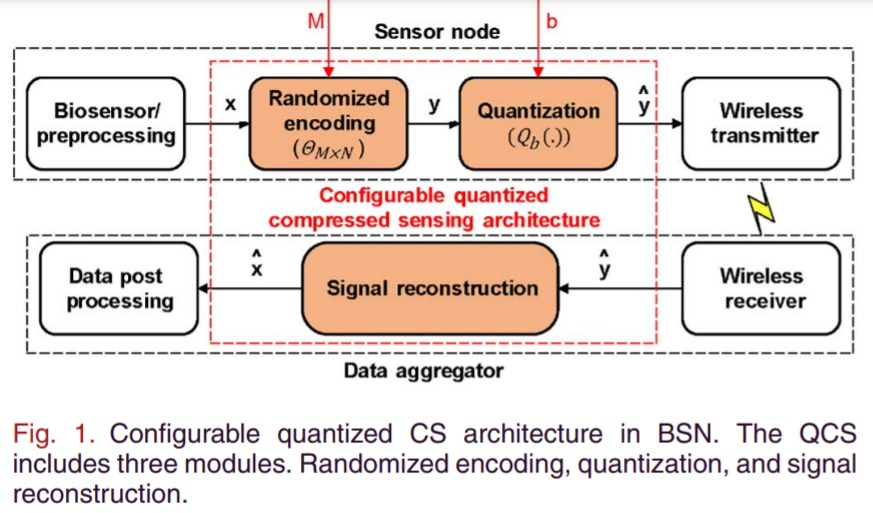
\includegraphics[width=400px]{Proposed Hardware architecture.png}
    \end{figure}
\end{center}
This paper combines two important ideas, one of which has been already discussed in the class: We define a parameter $M$, which denotes the rate at which the continuous stream of analog data is sampled and \textbf{then randomly encoded}. The second idea is that of \textbf{quantization}, which basically argues that analog signals should be \textbf{digitally quantized} based on a given \emph{bit resolution} $b$. It then proposes that we design a configurable hardware which takes as parameters $(M,b)$
\subsection{Reconstruction Techniques}
In this paper, the authors propose a novel algorithm they term \textbf{RapQCS}. The objective of this algorithm is to achieve as good a performance as possible, given that our energy budget (ie:- our computational resources) is constrained.

\newpage

\section{Problem 6}

Finally, a coding problem! Here, we have to simulate compressive sensing using artificial tools to mimic the hardware architecture and omp algorithm used for processing the snapshot. Let's begin!

\subsection{Generating the snapshot}

We begin with reading the \verb|cars.avi| video. We use the mmread functions provided to extract the required frames.
We convert them to grayscale using the \verb|rgb2gray()| function. This is followed by extracting the $120\times240$ subsection from each frame. Finally we have our frames, which look like this.

\begin{figure}[!h]
    \centering
    \includegraphics[width=200px]{"Frame 1.png"}
    \includegraphics[width=200px]{"Frame 2.png"}
    \includegraphics[width=200px]{"Frame 3.png"}
\end{figure}

Now, we use random bernoulli matrices to obtain the coded snapshots of the frames. Using the equation $E = \sum \limits_{t=1}^TC_t \cdot F_t$, and adding zero mean Gaussian random noise of standard deviation 2 to it, we get the following snapshot.


\begin{figure}[!h]
    \centering
    \includegraphics[width=300px]{"Coded_Snapshot_T=3.png"}
\end{figure}


\subsection{What are $A$ and $b$?}

We already have the coded snapshot. Assume that $E$ and $F_t$ are vectorised. This is as follows-
$$E = \sum \limits_{t=1}^TC_t \cdot F_t$$
We can convert the $C_t$ vector into a diagonal matrix, which will convert the dot-product into a matrix multiplication. Thus, we can say that $\Phi = diag(C_t)$. This gives us the following-
$$E = \sum \limits_{t=1}^T\Phi_t F_t$$
Finally, we know that $F_t$ is sparse in DCT basis, thus we have a DCT basis representation of the vector $F_t$.
Thus, we have, where $\Psi$ stands for the DCT matrix-
$$F_t = \Psi \Theta_t$$

Finally, we can combine the above equations to get-
$$E = \sum \limits_{t=1}^T\Phi_t \Psi \Theta_t$$

$$E = \boldsymbol{\Phi} \Psi \boldsymbol{\Theta}$$
where $\boldsymbol{\Phi}$ stands for $[\Phi_1|\Phi_2|\cdots|\Phi_T]$ and $\boldsymbol{\Theta}$ stands for $[\Theta_1^t|\Theta_2^t|\cdots|\Theta_T^t]^t$

Comparing with our equation, $Ax = b$, we have-
\begin{itemize}
    \item $b$ is the vector we have measured, and equals the vector $E$. It is of dimension $\mathbb{R}^{HW}$
    \item $x$ is the vector which we need to estimate. It is denoted by the vector $\boldsymbol{\Theta}$ and is basically the information about all the frames at once. Subseuently, it is of dimension $\mathbb{R}^{HWT}$.
    \item Finally, $A$ is the product of the matrices $\boldsymbol{\Phi}$ and $\Psi$. It is of dimension $\mathbb{R}^{HW \times HWT}$.
\end{itemize}

This way, we are able to convert our problem into the form $Ax=b$.

\subsection{Pathwise Reconstruction}

Now suppose we are dealing with patches instead of the whole image. Still, we have the same notion of $A$ and $b$.

Let the height and width of a patch be $h$ and $w$. Let the number of frames be T.

\begin{itemize}
    \item $A = \Phi \Psi $, where $A$ is of dimension $\mathbb{R}^{hw \times hwT}$.
    \item $\Phi$ is formed by horizontal concatenation of the diagonal matrices of the individual bernoulli coded matrices. It is of dimension $\mathbb{R}^{hw \times hwT}$.
    \item $\Psi$ is the DCT coefficient matrix, obtained by the following code in matlab-\\
    \begin{center}
        $\Psi =$ \verb|kron(dctmtx(p)', dctmtx(p)');|\\
    \end{center}
    This is because we need the 2D-DCT basis for reconstruction. Our signals are sparse in 2D-DCT.    
    \item $b$ again is the signal which we are measuring. It is of the dimension $\mathbb{R}^{hw}$.
    \item Finally, $x$ is the signal which we need to estimate. It is the combination of all the frames in question. Thus, it is of dimension $\mathbb{R}^{hwT}$.
\end{itemize}

\subsection{Error in OMP}

We have added a Gaussian noise of standard deviation 2 to each pixel of the coded snapshot. Let us deal with one patch at a time.

We know that the size of a patch = $m$ = $p*p$. Assuming that the error dies out within 3 standard deviations, we have the combined error of the image as follows-
$$ ||\eta||^2 = 9*\sigma^2*m $$.
According to Compressive sensing theory, our epsilon (error magnitude) should always be greater than the noise. Thus, with a patch size of 8*8 and noise from Gaussian distribution with std=2, we have-
$$ \epsilon \geq 9*4*64 $$
$$ \epsilon \geq 2304 $$

Since we are measuring the error in terms of norm($\eta$) rather than $|\eta|^2$, we have the error metric in the OMP as-
$$ ||\eta||_2 \leq \epsilon$$, where $\epsilon = \sqrt{2304} \approx 48$

Using this value of error term, we observe that the OMP algorithm completes in around 5-20 iterations for each image and we also get good results. This indicates the correctness of choosing a correct $\epsilon$.

\newpage
\subsection{Results}

\subsection{Coded Snapshots- Cars}
\begin{center}
    \includegraphics[width=200px]{"Coded_Snapshot_T=3.png"}
    \includegraphics[width=200px]{"Coded_Snapshot_T=5.png"}
    \includegraphics[width=200px]{"Coded_Snapshot_T=7.png"}
\end{center}

\subsection{Coded Snapshots- Flame}
\begin{center}
    \includegraphics[width=200px]{"fCoded_Snapshot_T=5.png"}
\end{center}
Results of T=3 and T=7 for the \verb|flame.avi| were not asked for, but are included in the results folder, if you wish to see them.

\newpage
\subsubsection{Cars, T=3}
We observed a Relative Mean Squared Error = 0.0111


\begin{figure}[H]
    \centering
    \includegraphics[width=200px]{"Frame 1.png"}
    \includegraphics[width=200px]{"Reconstruction- T=3, frame number=1.png"}
    \includegraphics[width=200px]{"Frame 2.png"}
    \includegraphics[width=200px]{"Reconstruction- T=3, frame number=2.png"}
    \includegraphics[width=200px]{"Frame 3.png"}
    \includegraphics[width=200px]{"Reconstruction- T=3, frame number=3.png"}
\end{figure}

\newpage

\subsubsection{Cars, T=5}

We observed a Relative Mean Squared Error = 0.0191


\begin{figure}[H]
    \centering
    \includegraphics[width=200px]{"Frame 1.png"}
    \includegraphics[width=200px]{"Reconstruction- T=5, frame number=1.png"}
    \includegraphics[width=200px]{"Frame 2.png"}
    \includegraphics[width=200px]{"Reconstruction- T=5, frame number=2.png"}
    \includegraphics[width=200px]{"Frame 3.png"}
    \includegraphics[width=200px]{"Reconstruction- T=5, frame number=3.png"}
    \includegraphics[width=200px]{"Frame 4.png"}
    \includegraphics[width=200px]{"Reconstruction- T=5, frame number=4.png"}
    \includegraphics[width=200px]{"Frame 5.png"}
    \includegraphics[width=200px]{"Reconstruction- T=5, frame number=5.png"}
\end{figure}

\newpage

\subsubsection{Cars, T=7}

We observed a Relative Mean Squared Error =  0.0277


\begin{figure}[H]
    \centering
    \includegraphics[width=200px]{"Frame 1.png"}
    \includegraphics[width=200px]{"Reconstruction- T=7, frame number=1.png"}
    \includegraphics[width=200px]{"Frame 2.png"}
    \includegraphics[width=200px]{"Reconstruction- T=7, frame number=2.png"}
    \includegraphics[width=200px]{"Frame 3.png"}
    \includegraphics[width=200px]{"Reconstruction- T=7, frame number=3.png"}
    \includegraphics[width=200px]{"Frame 4.png"}
    \includegraphics[width=200px]{"Reconstruction- T=7, frame number=4.png"}
    \includegraphics[width=200px]{"Frame 5.png"}
    \includegraphics[width=200px]{"Reconstruction- T=7, frame number=5.png"}

\end{figure}
\begin{figure}[H]
    \centering
    \includegraphics[width=200px]{"Frame 6.png"}
    \includegraphics[width=200px]{"Reconstruction- T=7, frame number=6.png"}
    \includegraphics[width=200px]{"Frame 7.png"}
    \includegraphics[width=200px]{"Reconstruction- T=7, frame number=7.png"}
\end{figure}

\newpage

\subsubsection{Flame, T=5}

We observed a Relative Mean Squared Error = 0.0012


\begin{figure}[H]
    \centering
    \includegraphics[width=200px]{"fFrame 1.png"}
    \includegraphics[width=200px]{"fReconstruction- T=5, frame number=1.png"}
    \includegraphics[width=200px]{"fFrame 2.png"}
    \includegraphics[width=200px]{"fReconstruction- T=5, frame number=2.png"}
    \includegraphics[width=200px]{"fFrame 3.png"}
    \includegraphics[width=200px]{"fReconstruction- T=5, frame number=3.png"}
    \includegraphics[width=200px]{"fFrame 4.png"}
    \includegraphics[width=200px]{"fReconstruction- T=5, frame number=4.png"}
    \includegraphics[width=200px]{"fFrame 5.png"}
    \includegraphics[width=200px]{"fReconstruction- T=5, frame number=5.png"}
\end{figure}

















\end{document}